% This file was created by tikzplotlib v0.9.8.
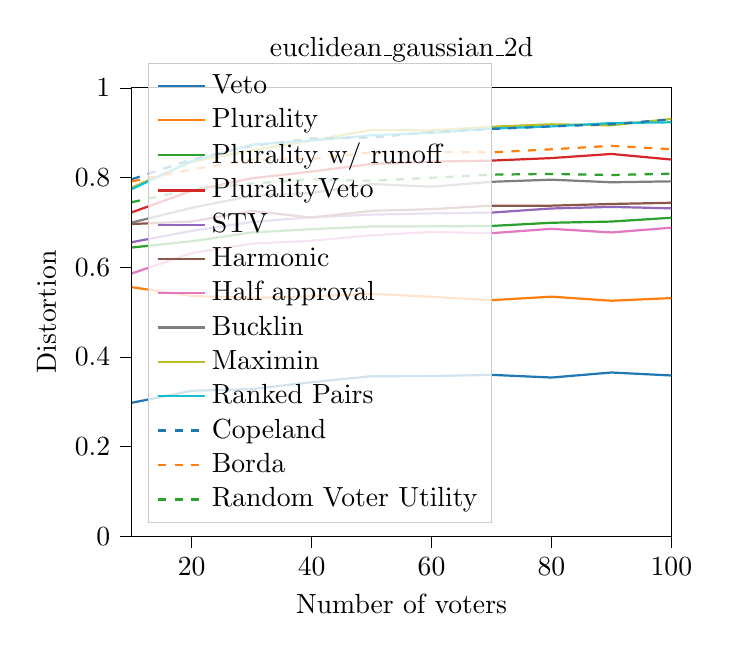
\begin{tikzpicture}

\definecolor{color0}{rgb}{0.12156862745098,0.466666666666667,0.705882352941177}
\definecolor{color1}{rgb}{1,0.498039215686275,0.0549019607843137}
\definecolor{color2}{rgb}{0.172549019607843,0.627450980392157,0.172549019607843}
\definecolor{color3}{rgb}{0.83921568627451,0.152941176470588,0.156862745098039}
\definecolor{color4}{rgb}{0.580392156862745,0.403921568627451,0.741176470588235}
\definecolor{color5}{rgb}{0.549019607843137,0.337254901960784,0.294117647058824}
\definecolor{color6}{rgb}{0.890196078431372,0.466666666666667,0.76078431372549}
\definecolor{color7}{rgb}{0.737254901960784,0.741176470588235,0.133333333333333}
\definecolor{color8}{rgb}{0.0901960784313725,0.745098039215686,0.811764705882353}

\begin{axis}[
legend cell align={left},
legend style={
  fill opacity=0.8,
  draw opacity=1,
  text opacity=1,
  at={(0.03,0.03)},
  anchor=south west,
  draw=white!80!black
},
tick align=outside,
tick pos=left,
title={euclidean\_gaussian\_2d},
x grid style={white!69.0196078431373!black},
xlabel={Number of voters},
xmin=10, xmax=100,
xtick style={color=black},
y grid style={white!69.0196078431373!black},
ylabel={Distortion},
ymin=0, ymax=1,
ytick style={color=black}
]
\addplot [thick, color0]
table {%
10 0.2976
20 0.3243
30 0.3282
40 0.3434
50 0.3569
60 0.3571
70 0.3599
80 0.3539
90 0.3651
100 0.3585
};
\addlegendentry{Veto}
\addplot [thick, color1]
table {%
10 0.5554
20 0.536
30 0.5314
40 0.535
50 0.5408
60 0.5338
70 0.5265
80 0.5343
90 0.5252
100 0.5311
};
\addlegendentry{Plurality}
\addplot [thick, color2]
table {%
10 0.6439
20 0.6578
30 0.6775
40 0.6848
50 0.6908
60 0.6911
70 0.692
80 0.6991
90 0.7018
100 0.7103
};
\addlegendentry{Plurality w/ runoff}
\addplot [thick, color3]
table {%
10 0.7223
20 0.7705
30 0.7983
40 0.8134
50 0.8303
60 0.8355
70 0.8378
80 0.8434
90 0.8526
100 0.8401
};
\addlegendentry{PluralityVeto}
\addplot [thick, color4]
table {%
10 0.6558
20 0.681
30 0.7007
40 0.7115
50 0.7172
60 0.72
70 0.7218
80 0.731
90 0.7345
100 0.7313
};
\addlegendentry{STV}
\addplot [thick, color5]
table {%
10 0.6963
20 0.7019
30 0.7254
40 0.7106
50 0.7257
60 0.7294
70 0.7373
80 0.7373
90 0.741
100 0.7437
};
\addlegendentry{Harmonic}
\addplot [thick, color6]
table {%
10 0.586
20 0.6315
30 0.6525
40 0.6591
50 0.6712
60 0.6786
70 0.6759
80 0.6856
90 0.6775
100 0.6881
};
\addlegendentry{Half approval}
\addplot [thick, white!49.8039215686275!black]
table {%
10 0.6996
20 0.7325
30 0.7592
40 0.7656
50 0.7856
60 0.7795
70 0.7905
80 0.7952
90 0.7894
100 0.7915
};
\addlegendentry{Bucklin}
\addplot [thick, color7]
table {%
10 0.7775
20 0.8352
30 0.8606
40 0.8825
50 0.9062
60 0.9049
70 0.9132
80 0.9187
90 0.9165
100 0.9307
};
\addlegendentry{Maximin}
\addplot [thick, color8]
table {%
10 0.7742
20 0.8368
30 0.8734
40 0.8825
50 0.8942
60 0.8995
70 0.9092
80 0.9141
90 0.9215
100 0.9232
};
\addlegendentry{Ranked Pairs}
\addplot [thick, color0, dashed]
table {%
10 0.7962
20 0.8403
30 0.8705
40 0.8873
50 0.889
60 0.9015
70 0.9083
80 0.9141
90 0.9188
100 0.9297
};
\addlegendentry{Copeland}
\addplot [thick, color1, dashed]
table {%
10 0.7913
20 0.8183
30 0.8391
40 0.8415
50 0.8563
60 0.8572
70 0.856
80 0.863
90 0.8707
100 0.8632
};
\addlegendentry{Borda}
\addplot [thick, color2, dashed]
table {%
10 0.745
20 0.7735
30 0.7867
40 0.7961
50 0.7926
60 0.7996
70 0.8064
80 0.8081
90 0.8056
100 0.8086
};
\addlegendentry{Random Voter Utility}
\end{axis}

\end{tikzpicture}
